\chapter{Model and methods}
\label{chap:modmet}
\section{Modeling System description}
\label{sec:modeldes}
(What did Johanne and Kjetil think was important enough to write about in their thesees?)

To produce results for the thesis, a formulation of the Weather Research and Forecasting (WRF) Model called the Advanced Research WRF (ARW) has been used, Version 3.6.1, released in April 2014. The model is developed at the National Centre for Atmospheric Research (NCAR) in Boulder, Colorado. The ARW model is the first fully compressible conservative form nonhydrostatic model designed for both research and operational numerical weather prediction (NWP) applications~\citep{Skamarock2008}. 

As can be seen from figure~\ref{fig:wrfflowchart} the WRF Modeling System consists of four major programs~\citep{Wang2012}:
\begin{itemize}
\item The WRF Prepocessing System (WPS)
\item WRF-Data Assimilation (WRF-DA)
\item ARW solver
\item Post-processing \& Visualization tools
\end{itemize}

WPS is used primarily for real data simulations~\citep{Wang2015}, like the study presented in this thesis. Its functions include defining simulation domains, interpolating terrestrial data and degribbing and interpolating meteorological data from another model to this simulation domain~\citep{Wang2015}. WRF-DA is optional and can be used to ingest observations into the interpolated analyses created by WPS~\citep{Wang2015}, but was not used in this study. The ARW solver is the key component of the modeling system, which is composed of several intialization programs for idealized, and real-data simulations, and the numerical integration program~\citep{Wang2015}. Fully compressible nonhydrostatic equations with hydrostatic options, regional and global applications, complete coriolis and curvature terms and that vertical grid-spacing can vary with height are among the WRF models key features according to~\cite{Wang2015}.

\begin{figure}
\centering
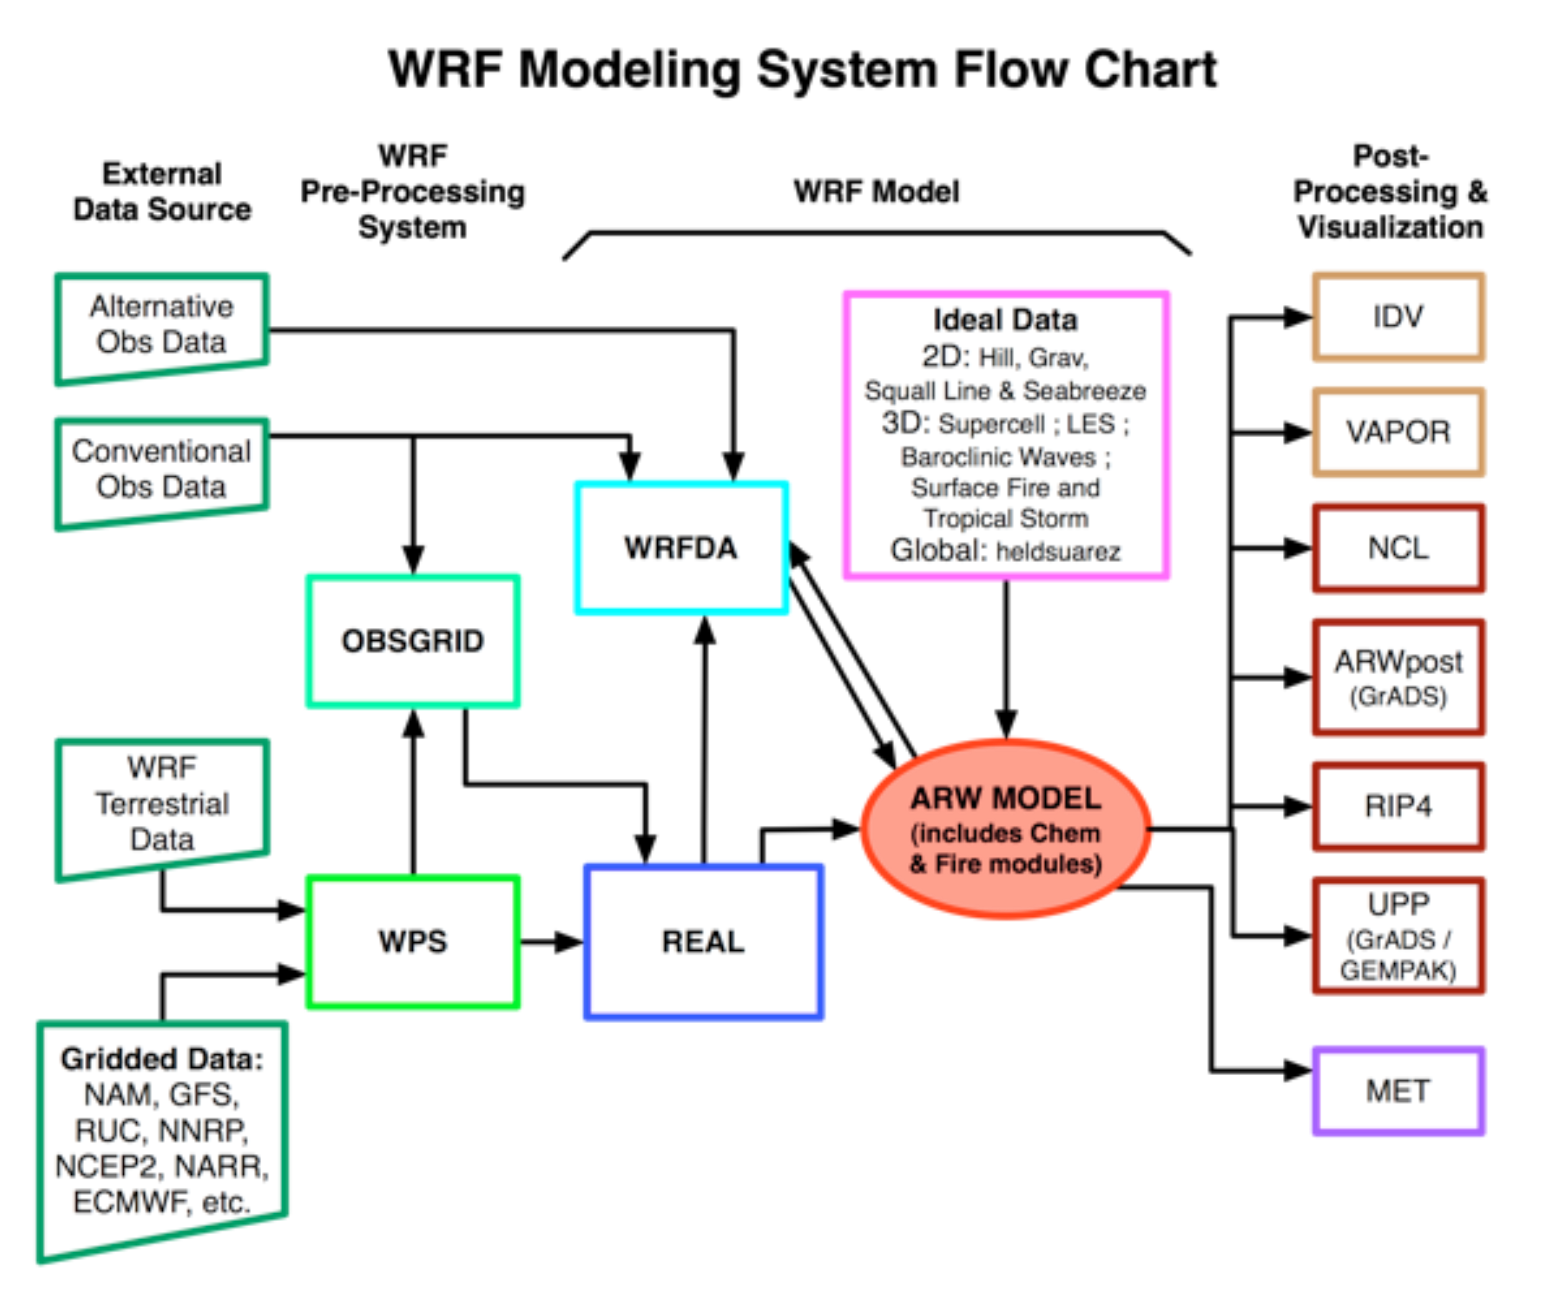
\includegraphics[width=\textwidth]{wrfflowchart}
\caption{Flowchart for the WRF ARW Modeling System Version 3. From~\cite{Wang2015}.}
\label{fig:wrfflowchart}
\end{figure}

%Any detailed information on the model, presented in this section is based on the Article by~\cite{Skamarock2008} unless otherwise stated.

The continuous equations solved in the ARW model are the Euler equations cast in a flux form where the vertical coordinate, $\eta$, is defined by a normalized hydrostatic pressure,
\begin{equation}
\eta = (p_h - p_{ht})/\mju 
\end{equation}
where $\mju = (p_{hs} - p_{ht})$~\citep{Skamarock2008}. $p_h$ is the hydrostatic component of the pressure and $p_{hs}$ and $p_{ht}$ are the values of the hydrostatic pressure in a dry atmosphere at the surface and top boundaries respectively~\citep{Skamarock2008}.

The vertical coordinate is the traditional $\sigma$ coordinate used in many hydrostatic atmospheric models, shown in a diagram in figure~\ref{fig:sigma}.

\begin{figure}
\centering
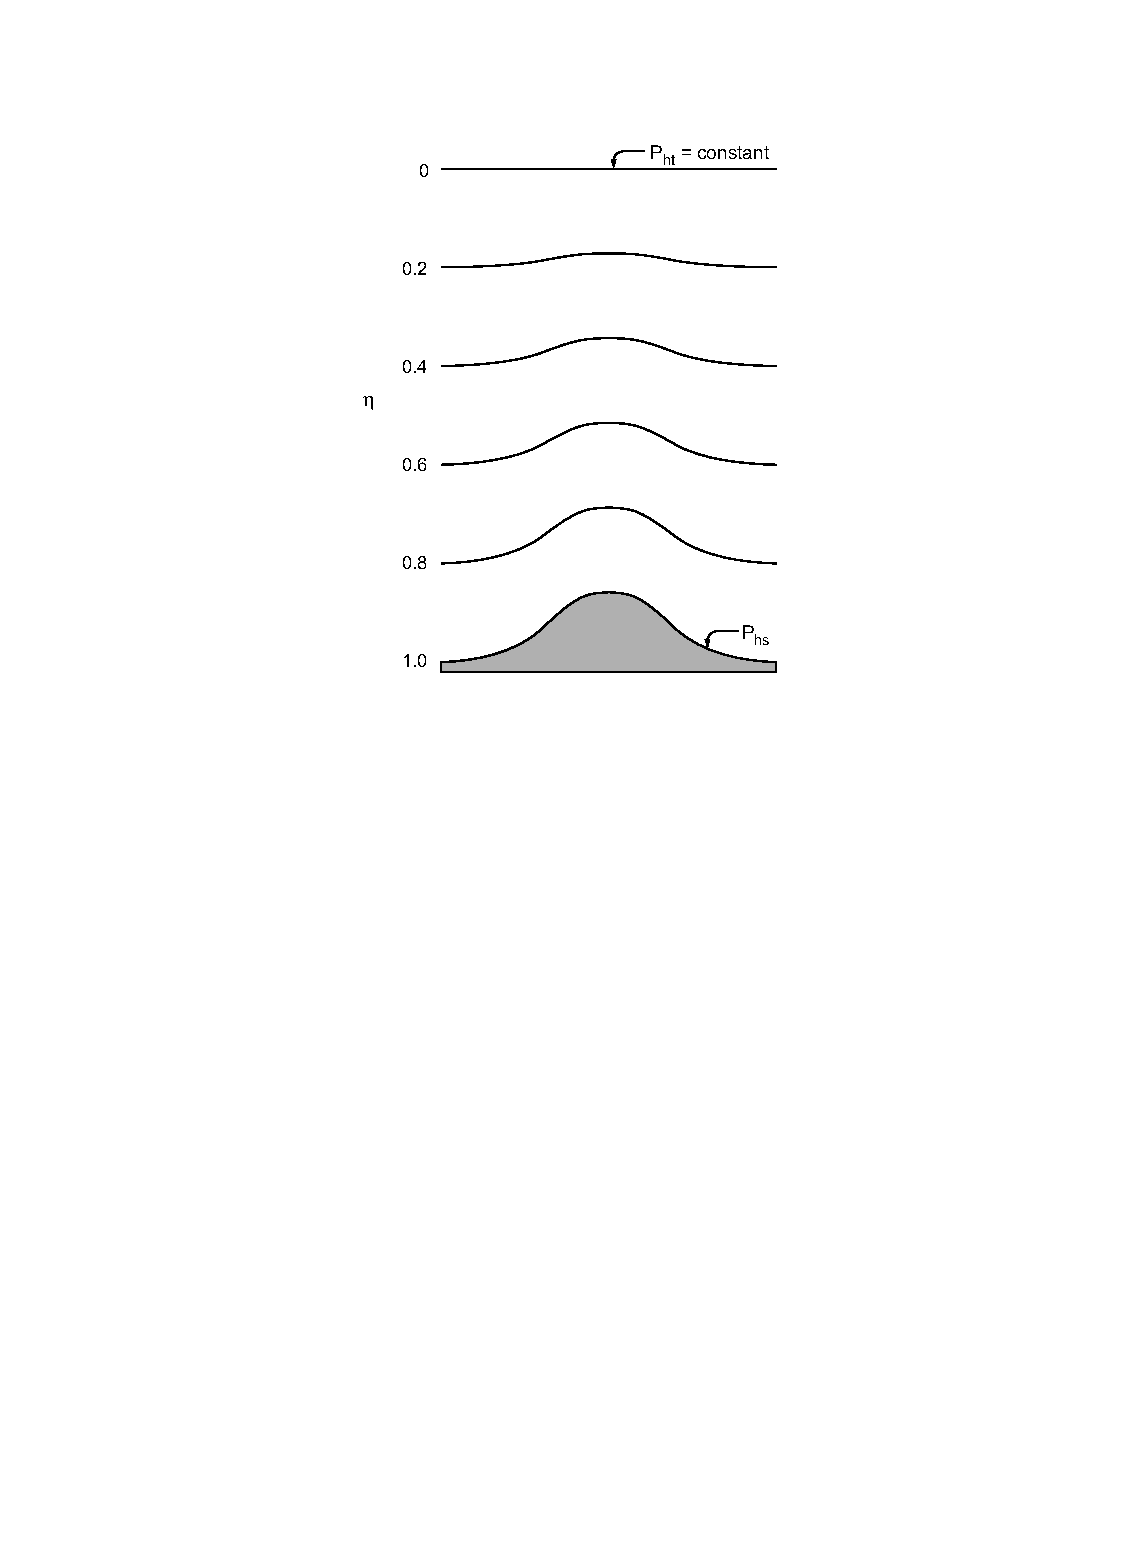
\includegraphics[scale=1]{sigma.pdf}
\caption{This figure is shown as presented in~\cite{Skamarock2008}, and is a schematic of the terrain following a $\sigma$ coordinate. $P_{hs}$ and $P_{ht}$ is the hydrostatic pressure at the surface and the top respectively.}
\label{fig:sigma}
\end{figure}

\section{Schemes}
\label{sec:schemes}
The ARW model offers a wide selection of schemes to treat different physics that one wants represented in the model. The schemes treat the physics slightly differently and some schemes are better for certain horisontal and vertical resolutions than others, so one needs to be careful when choosing how the model is to treat the physics. For my thesis, the especially relevant scheme to mention is the cloud microphysics scheme that I chose, which is the aerosol-aware scheme described in~\cite{Thompson2014} which is a development of the bulk microphysisc scheme described in~\cite{Thompson2008}, to include aerosols and scavenging of them. The scheme is a true double moment scheme and therefore treats cloud water, cloud ice, rain and snow in a complex and detailed way(@???litt vagt og rart å skrive)~\cite{Thompson2014}. At the time of writing, the only radiation schemes that make use of the effective radii are the Rapid Radiative Tranfer Model (RRTM) for General Circulation Models (GCMs) (RRTMG) radiation schemes~\cite{@authorsRRTMG} for both SW and LW. These were therefore used in combination with the aerosol-aware cloud microphysics scheme.

\subsection{The aerosol-aware scheme}
The microphysics option 28~\citep{Thompson2014} is built on the schematic shown in figure~\ref{fig:microphysics}. It is a double moment scheme, which means it computes both mixing ratios and number concentrations for the same water species (hydrometeors). 

\begin{figure}
\centering
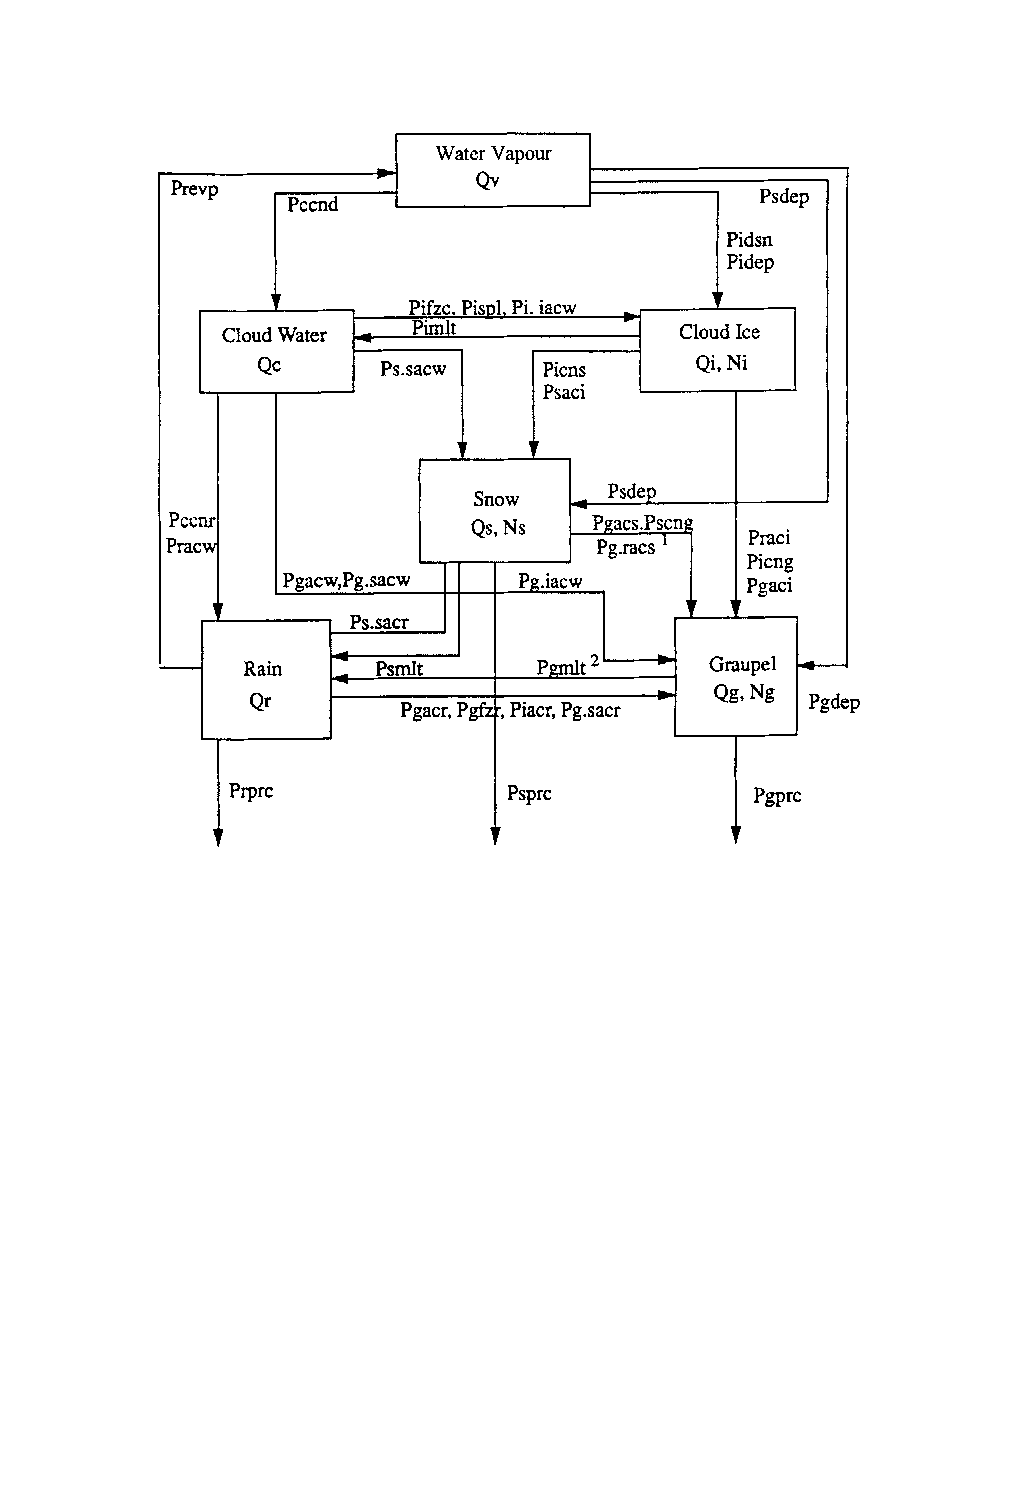
\includegraphics[scale=0.8]{microphysics.pdf}
\caption{Cloud microphysical parameterization scheme typically used i NWP models as shown in~\cite{Reisner1998}. A full list of the acronyms used in the schematic can be found in~\cite{Reisner1998}.}
\label{fig:microphysics}
\end{figure}

Write more about this figure!

\section{Model setup}
\label{sec:modelsetup}
@Area description. Sea names: Beaufort and ??. By Canada and Alaska, this is because data from the area has been used for research by others @citations. The area is not ice free any part of the year @cite, and provides a good place to simulate cloud and sea ice interaction.
\\
I ran ARW with a horisontal resolution of 4 km, and 72 vertical layers. This resolution is sufficient to resolve clouds @citation. 300$\cdot$ 300 gridpoints, with 4 km spacing, between .
\\
I call the vertical layers in the ARW model eta levels, because of the choice of $\eta$ as the vertical coordinate. These levels have uneven vertical spacing. Since the level height is dependent on pressure, the height varies in both time and space. Consequently the levels in the lower troposphere are closer to each other than higher up in the troposphere. Therefore the low clouds in the area can be resolved. (@How close? what heights??)
\\
The sea ice in the area was removed by editing the input file constructed? built? by WPS and real.exe, to get results to compare with results from runs with ice.
\\
From diminishing sea ice we might experience an increase in sea traffic, which would lead to an increase in aerosol content in otherwise clean air @citation. To include increase in aerosol concentrations due to lack of sea ice I used the microphysics scheme developed by Greg Thompson and Trude Eidhammer described in~\cite{Thompson2014}.
\\
The scheme uses a monthly mean for aerosol number concentrations derived from multi-year (2001-2007) global model simulations @citationColarco2010??(det har de cita) in which particles and their precursors are emitted by natural and anthropogenic sources and are explicitly modeled with multiple size bins for multiple species of aerosols by the Goddard Chemistry Aerosol Radiation and Transport (GOCART) model (@desiterteGinoux2001)~\citep{Thompson2014}.
\\
Choice of schemes and reasons should be presented. As should hos WPS and real.exe and wrf.exe works. At least short about what they do and contribute with to get to the end results. Explain some of the improvements in the micro physics scheme in combination with the revised radiation schemes (RRTMG for SW and LW).

\section{Model runs}
\begin{table}[H]
\centering
\caption{Table showing the name of the runs and what is included}
%Caption could say: Table showing the names of the runs and if they have sea ice or not, and if the aerosol concentration has been increased. All the runs have the same horisontal resolution of 4kmx4km, dimensons 300x300, vertical layers 72 and time step 24 s.
\label{tab:runs} 
\begin{tabular}{L{2.3cm} L{2.3cm} L{2cm} L{1.5cm} L{1cm} L{1.5cm} L{3cm}}
\centering
Name & Horisontal resolution & Dimensions & Vertical layers & $\Delta$t & Sea ice & Aerosol concentration\\ \hline
control & 4~km x 4~km & 300 x 300 & 72& 24~s & initial & control \\
NoIce & 4~km x 4~km & 300 x 300 & 72 & 24~s & removed & control \\
IncAero & 4~km x 4~km & 300 x 300 & 72 & 24~s & initial & control x 100 \\
IncAeroNoIce & 4~km x 4~km & 300 x 300 & 72 & 24~s & removed & control x 100 \\
\end{tabular}
\end{table}

Which table?

\begin{table}[H]
\centering
\caption{Caption could say: Table showing the names of the runs and if they have sea ice or not, and if the aerosol concentration has been increased. All the runs have the same horisontal resolution of 4kmx4km, dimensons 300x300, vertical layers 72 and time step 24 s.}
\label{tab:runs} 
\begin{tabular}{L{2.3cm} L{2cm} L{3cm}}
\centering
Name & Sea ice & Aerosol concentration\\ \hline
control & initial & control \\
NoIce & removed & control \\
IncAero & initial & control x 100 \\
IncAeroNoIce & removed & control x 100 \\
\end{tabular}
\end{table}

\subsection{Manipulation of input files}
wrfinput_d01 and wrfbdy_d01 are input files made by wrf_init.exe
To run the model without ice and with an increased number of aerosols I manipulated the input files for WRF. I used a netCDF Operator (NCO) tool, ncap2. This allowed me do manipulate the netCDF files from my terminal window in the folder where they were located.
Elaborate on removal or placing of sea ice. Elaborate on multiplying the aerosol number concentration with a factor 10. By use of ncap2 from NetCDF (NCO).

\subsection{Changed ice run}
The sea ice variable in the wrfinput_d01 file was simply multiplied by 0 in every gridpoint and by that removed.
Removed ice from the input file for the model run by using NCO and ncap2. The point of this is to compare the run with no ice to the control run, and see if there are any changes to the cloud properties.

\subsection{Changed aerosols run}
The increase in aerosol concentration was a bit more complicated, but the same method. The number of water and ice friendly aerosols were multiplied by 100 and so were their tendencies and respective concentrations at the boundaries of the area. %wrfbdy is a lateral boundary file, contains the WRF lateral boundary conditions~\citep{Wang2015}.
The goal is to find changes in cloud properties compared to those in the control run, for that purpose the aerosol concentration was multiplied by a factor of 100. Hoping to get a signal.

\section{Input data}
The model runs were initialized with data downloaded from the European Centre for Medium-Range Weather Forecasts (ECMWF).%was downloaded from their site and used as input for initial and boundary?? conditions.
The downloaded data is from the ERA-Interim dataset, which is a global atmospheric reanalysis from 1979 to present and continues to be updated in real time.%~\cite{ecmwf}.@make bib for ecmwf
Through WPS the data from ERA-Interim was interpolated over a the grid, with a 2 degree minute spacing between the points, to be used to initialize the model. The data is in 6-hourly atmospheric fields on pressure levels, for the first five days of September 2012, which was the period the model was run for.

\section{Processing of the results}
Figures presented in my thesis, I made (unless other is stated) by use of National Centre for Atmospheric Research (NCAR) Command Language (NCL) and MatLab. For the NCL scripts I found a lot of help and inspiration from the example scripts for WRF-users available at (URL for examples).

I made some figures with NCL, but most with MatLab provided by the University. Most figures that are not over a map were made with MatLab. MathWorks, it is very useful and easy to use.